\documentclass[letterpaper,12pt]{article}
\usepackage{geometry}
\usepackage{setspace}
\usepackage{tabularray}
\usepackage{array}
\usepackage{multicol}
\usepackage{graphicx}
\usepackage{float}
\geometry{margin=2.5cm}
\usepackage[utf8x]{inputenc}
\usepackage[english]{babel}
\usepackage{csquotes}
\usepackage[T1]{fontenc}
\fontfamily{phv}\selectfont
\usepackage[]{fancyhdr}
\pagestyle{fancy}
\setlength{\headheight}{13pt}
\setlength{\tabcolsep}{1em}
\title{\large{Acme Video Store database proposal}}
\author{Alberth Matos}
\date{\today}
\NewTblrTheme{fancy}{
	\SetTblrStyle{firsthead}{font=\bfseries}
}
\UseTblrLibrary{booktabs}
\begin{document}

% Clear all headers and footers (see also \fancyhf{})
\fancyhead{}
\fancyhead[R]{\small Alberth Matos}
\fancyhead[L]{\small CMIS 320}
\fancyhead[C]{\small Project 2}

\maketitle

\section{Description}
This database system will help \emph{Acme Video Rental} modernize their business by digitizing a currently manual process, which will help \emph{Acme Video Rental} be more effective, efficient, and better serve their customers.  The database will collect information on Actors, Movies, Directors, Producers, movie genres, release years, and awards, mapping those entities with relationships such that \emph{Acme Video Rental} staff can help customers by directing them to what movies have won Academy Awards, which movies feature which actors and actresses, which films were produced by certain producers, or movies within certain genres that were released in a given year.

In order to help \emph{Acme Video Rental} better their costs, the database system will also take in electronic data provided by various suppliers, so that \emph{Acme Video Rental} staff can search their suppliers' catalogues to identify which supplier offers the best price for a specific movie and format (i.e., ``Gone with the Wind'' in VHS may be one price, but the DVD may be a different price.).  By querying the database for the price of a specific movie, \emph{Acme Video Rental} can determine which supplier offers the lowest cost.

The database system will also help \emph{Acme Video Rental} track their customers by recording when a Movie is rented, and whether any fees are due as a result of either damaged, late, or, in the case of VHS tapes, a failure to rewind the tape before it is returned.  This will also provide a benefit to \emph{Acme Video Rental}'s customers, who will be able to track what movies they have rented, and possibly identify previously unknown preferences on genres, directors, actors and actresses.  As an additional benefit, \emph{Acme Video Rental} will also be able to offer ``Family Accounts'' so that other members of a customer's family will be able to consolidate billing under a single individual.  This also provides a measure of parental controls, as ``Family Account'' members can be restricted to only rent movies under a predefined rating (That is, a restricted child account should not be able to rent an 'R' or 'MA' movie).

\section{Data Model}
\subsection{Entities and preliminary attributes}
\begin{itemize}
	\item AAMapper: Actor to Award Mappers
	      \begin{itemize}
		      \item Attributes: MapperID (key), ActorID (foreign key referencing Actor/Actress), AwardID (foreign Key referencing Award)
	      \end{itemize}
	\item Actors: Represents an Actor or Actress in a movie.
	      \begin{itemize}
		      \item Attributes: ActorID (key), Name (Given and Family names, that is, First and Last names, in separate fields)
	      \end{itemize}
	\item Addresses: Represents an address belonging to a customer, distributor, or other entity.
	      \begin{itemize}
		      \item Attributes: AddressID (key), Street Address (2 lines), Suite, City, State, Postal Code
	      \end{itemize}
	\item AMMapper: Actor to Movie Mapper.
	      \begin{itemize}
		      \item Attributes: MapperID (key), ActorID (FK), MovieID (FK)
	      \end{itemize}
	\item Awards: Represents an Academy Award won by an actor/actress, director, or movie.
	      \begin{itemize}
		      \item Attributes: AwardID (key), Name, Award won (was the award won, or was it a nomination only), Award year
	      \end{itemize}
	\item Customers: Represents a customer of \emph{Acme Video Rental}.
	      \begin{itemize}
		      \item Attributes: CustomerID (key), Name, Address (FK), Phone Number, Email address, Parent ID (for sub-accounts), Restricted (for child accounts)
	      \end{itemize}
	\item DMMapper: Director to Movie Mappers.
	      \begin{itemize}
		      \item Attributes: MapperID (key), DirectorID (FK), MovieID (FK)
	      \end{itemize}
	\item DAMapper: Director to Award Mappers.
	      \begin{itemize}
		      \item Attributes: MapperID (key), DirectorID (FK), AwardID (FK), Award Won (FK)
	      \end{itemize}
	\item Directors: A director of a movie.
	      \begin{itemize}
		      \item Attributes: DirectorID (key), Name
	      \end{itemize}
	\item Distributors: An entity that sells movies in different media to wholesale customers.
	      \begin{itemize}
		      \item Attributes: DistributorID (key), Name, Billing Address (FK), Returns Address (FK), Phone Number, Discount Rate
	      \end{itemize}
	\item DistCat: Distributor catalogue
	      \begin{itemize}
		      \item Attributes: DistCatID (key), Distributor (FK), Movie (FK), Price, Medium, Distributor Serial Number
	      \end{itemize}
	\item Fees: Different fees that might apply to a rental.
	      \begin{itemize}
		      \item Attributes: FeeID (key), Fee Description, Fee Cost, Fee start date, Fee end date
	      \end{itemize}
	\item GMMapper: Genre to Movie Mapper
	      \begin{itemize}
		      \item Attributes: GMMapperID (key), Genre (FK), Movie (FK)
	      \end{itemize}
	\item Genres: Genre of the movie
	      \begin{itemize}
		      \item Attributes: GenreID (key), Genre
	      \end{itemize}
	\item Media: A VHS tape or DVD disc.
	      \begin{itemize}
		      \item Attributes: MediumID (key), Medium Type, Movie ID (FK), Acme Inventory ID, Distributor (FK), Distributor Serial Number, Distributor Movie ID, Rental Price
	      \end{itemize}
	\item Movies: A film.
	      \begin{itemize}
		      \item Attributes: MovieID (key), Acme Movie ID, Title, Duration, Rating, Genre (FK)
	      \end{itemize}
	\item PMMapper: Producer to Movie Mappers
	      \begin{itemize}
		      \item Attributes: PMMapperID (key), Producer (FK), Movie (FK)
	      \end{itemize}
	\item Producers: A person who produces a movie.
	      \begin{itemize}
		      \item Attributes: ProducerID (key), Name, Production Company
	      \end{itemize}
	\item Rentals: Individual rentals by customers.
	      \begin{itemize}
		      \item Attributes: Rental ID (key), Rental Date, Scheduled Return Date, Was Movie Returned, Customer (FK), Medium (FK), Discount Applied, Late Fee (FK), Damage Fee (DK), Rewind Fee (FK), Tax charged
	      \end{itemize}
\end{itemize}
\subsection{Relationship Sentence Pairs}
A customer may rent one or more movie media.\\
Media may be rented by one or more customers.\\
\\
A medium is a specific instance of a movie on VHS or DVD.\\
Movies may be available in one or more media.\\
\\
A movie may have one or more actors/actresses.\\
An actor/actress may appear in one or more movies.\\
\\
A movie may have one or more directors.\\
A director may direct one or more movies.\\
\\
A movie may have one or more producers.\\
A producer may produce one or more movies.\\
\\
A movie may win zero to many Academy Awards.\\
An Academy Award may be won by one movie.\\
\\
A movie's director(s) may win zero or one Academy Awards.\\
An Academy Award may be won by one movie's director(s).\\
\\
One movie's actor may win zero or one Academy Awards.\\
An Academy Award may be won by one movie's actor.\\
\\
One movie's actress may win zero or one Academy Awards.\\
An Academy Award may be won by one movie's actress.\\
\\
A movie must have one or more genres.\\
A genre can be shared by many movies.\\
\\
A customer may have only one address.\\
An address may belong to multiple customers.\\
\\
A distributor may distribute many movies media.\\
A movie's medium may be sold by one or more distributors.\\
\\
A distributor may have multiple addresses.\\
An address can belong to only one distributor\\
\\
A customer may be a sub-account of another customer.\\
A sub-account can only belong to one other customer.\\
\\
A distributor must produce a distributor catalog.\\
A distributor catalog must belong to a distributor.\\
\\
A medium may appear in one or more distributor catalogs.\\
A distributor catalog may contain many media.\\

\section{ER Diagrams}
\subsection{Overview}
As an overview of the physical model, here is the complete full data model for this database system.  For details on components of the data model, as well as more legible images, please see the individual sections below.
\begin{figure}[H]
	\centering
	\caption{Full Data Model}
	\label{fig:Full_Data_Model}
	\includegraphics[width=1.0\linewidth]{Data Model.png}
\end{figure}

\subsection{Bridge Tables}
Bridge tables are used to connect together tables that would otherwise have a many-to-many relationship.
\begin{figure}[H]
	\centering
	\caption{AAMapper: Connecting Actors/Actresses to Awards}
	\label{fig:AAMapper}
	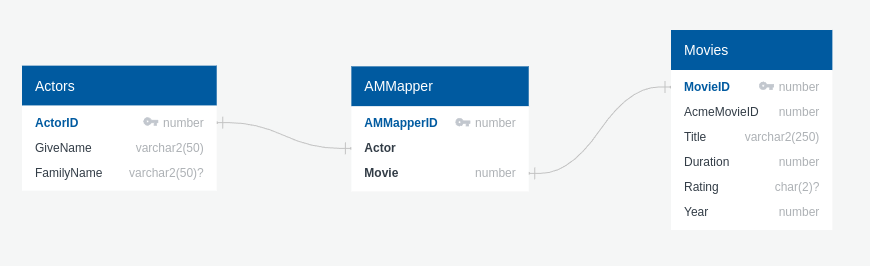
\includegraphics[width=1.0\linewidth]{AAMapper - Actors - Awards.png}
\end{figure}
\begin{figure}[H]
	\centering
	\caption{AMMapper: Map Actors/Actresses to Movies}
	\label{fig:AMMapper}
	\includegraphics[width=1.0\linewidth]{"AMMapper - Actors - Movies.png"}
\end{figure}
\begin{figure}[H]
	\centering
	\caption{DAMapper: Map Directors to Awards}
	\label{fig:DAMapper}
	\includegraphics[width=1.0\linewidth]{"DAMapper - Directors - Awards.png"}
\end{figure}

\section{Metadata}
\begin{longtblr}[
		theme = fancy,
		label=none,
		caption = {Acme Video Rental}
	]{
		colspec = {XXX[-1,c]XX},
		width = 0.95\linewidth,
		rowhead = 1
	}
	\toprule[2pt]
	Entity       & Attributes        & PK/FK & Data Types    & Description                                                   \\
	\midrule
	AAMapper     & AAMapperID        & PK    & NUMBER        & Primary Key for Actor to Award Mapper. Not null.              \\
	             & Actor             & FK    & NUMBER        & FK for Actors.ActorID.                                        \\
	             & Award             & FK    & NUMBER        & FK for Awards.AwardID.                                        \\
	\\
	Actors       & ActorID           & PK    & NUMBER        & Primary Key for Actor Entity. Not null.                       \\
	             & GivenName         &       & VARCHAR2(50)  & Actor's/Actress' Given Name. Not null.                        \\
	             & FamilyName        &       & VARCHAR2(50)  & Actor's/Actress' Family Name.                                 \\
	\\
	Addresses    & AddressID         & PK    & NUMBER        & Primary Key for Addresses. Not Null.                          \\
	             & StreetAddress1    &       & VARCHAR2(50)  & Street Address. Not null.                                     \\
	             & StreetAddress2    &       & VARCHAR2(50)  & Street Address, line 2.                                       \\
	             & Suite             &       & VARCHAR2(20)  & Suite Number/Code.                                            \\
	             & City              &       & VARCHAR2(50)  & City name. Not null.                                          \\
	             & State             &       & VARCHAR2(20)  & State name. Not null.                                         \\
	             & PostalCode        &       & VARCHAR2(20)  & Postal Code. Not null.                                        \\
	             & Country           & FK    & CHAR(2)       & FK for Countries.CountryID                                    \\
	\\
	AMMapper     & AMMapperID        & PK    & NUMBER        & Primary Key for Actor to Movie Mapper. Not null.              \\
	             & Actor             & FK    & NUMBER        & FK for Actors.ActorID.                                        \\
	             & Movie             & FK    & NUMBER        & FK for Movies.MovieID.                                        \\
	\\
	Awards       & AwardID           & PK    & NUMBER        & Primary Key for Award.                                        \\
	             & AwardName         &       & VARCHAR2(20)  & Name of award.                                                \\
	             & AwardWon          &       & BOOLEAN       & Was nominated or won award.                                   \\
	\\
	Customers    & CustomerID        & PK    & NUMBER        & PK for Customer Entity. Not null.                             \\
	             & GivenName         &       & VARCHAR2(50)  & Customer Given Name. Not null.                                \\
	             & FamilyName        &       & VARCHAR2(50)  & Customer Family Name.                                         \\
	             & Address           & FK    & NUMBER        & FK for Addresses.AddressID.                                   \\
	             & PhoneNumber       &       & NUMBER        & Telephone Number. Not null.                                   \\
	             & Email             &       & VARCHAR2(50)  & Email Address.                                                \\
	             & ParentID          & FK    & NUMBER        & FK for Customers.Customer. Used to track ``family'' accounts. \\
	             & Restricted        &       & BOOLEAN       & Flag for a restricted account.                                \\
	\\
	DAMapper     & DAMapperID        & PK    & NUMBER        & Primary Key for Director to Award Mapper. Not null.           \\
	             & Director          & FK    & NUMBER        & FK for Directors.DirectorID                                   \\
	             & Award             & FK    & NUMBER        & FK for Awards.AwardID.                                        \\
	\\
	Directors    & DirectorID        & PK    & NUMBER        & Primary Key for Director Entity. Not null.                    \\
	             & GivenName         &       & VARCHAR2(50)  & Director Given (First) Name. Not null.                        \\
	             & FamilyName        &       & VARCHAR2(50)  & Director Family (Last) Name.                                  \\
	\\
	Distributors & DistributorID     & PK    & NUMBER        & Primary Key for Distributors. Not null.                       \\
	             & DistributorName   &       & VARCHAR2(50)  & Distributor Name. Not null.                                   \\
	             & BillingAddress    & FK    & NUMBER        & FK for Addresses.AddressID.                                   \\
	             & ReturnsAddress    & FK    & NUMBER        & FK for Addresses.AddressID.                                   \\
	             & PhoneNumber       &       & NUMBER        & Distributor Phone Number. Not null.                           \\
	             & EmailAddress      &       & VARCHAR2(50)  & Email Address.                                                \\
	             & Discount          &       & NUMBER        & Discount rate offereed.                                       \\
	\\
	DistCat      & DistCatID         & PK    & NUMBER        & Primary key for Distributor Catalogue ID. Not null.           \\
	             & Distributor       & FK    & NUMBER        & FK for Distributors.DistributorID.                            \\
	             & Movie             & FK    & NUMBER        & FK for Movies.MovieID.                                        \\
	             & Price             &       & Number        & Catalogue Price.                                              \\
	             & Medium            &       & VARCHAR2(5)   & Medium Type.                                                  \\
	             & DistributorSerial &       & VARCHAR2(50)  & Distributor Serial Number.                                    \\
	\\
	DMMapper     & DMMapperID        & PK    & NUMBER        & Primary Key for Director to Movie Mapper. Not null.           \\
	             & MovieID           & FK    & NUMBER        & FK for Movies.MovieID.                                        \\
	             & DirectorID        & FK    & NUMBER        & FK for Directors.DirectorID.                                  \\
	\\
	Fees         & FeeID             & PK    & NUMBER        & PK for Fee.                                                   \\
	             & Fee               &       & VARCHAR2(20)  & Type of Fee.                                                  \\
	             & FeeCost           &       & NUMBER        & Cost of Fee.                                                  \\
	             & FeeStart          &       & DATE          & Date Fee effective.                                           \\
	             & FeeEnd            &       & DATE          & Date Fee expired.                                             \\
	\\
	Genres       & GenreID           & PK    & NUMBER        & Primary Key for Genre. Not null.                              \\
	             & Genre             &       & VARCHAR2(20)  & Genre Description.                                            \\
	\\
	GMMapper     & GMMapperID        & PK    & NUMBER        & Primary Key for Genre to Movie Mapper. Not null.              \\
	             & Genre             & FK    & NUMBER        & FK for Genres.GenreID.                                        \\
	             & Movie             & FK    & NUMBER        & FK for Movies.MovieID.                                        \\
	\\
	MAMapper     & MAMapperID        & PK    & NUMBER        & Primary Key for Movie to Award Mapper. Not null.              \\
	             & Award             & FK    & NUMBER        & FK for Awards.awardID.                                        \\
	             & Movie             & FK    & NUMBER        & FK for Movies.MovieID.                                        \\
	\\
	Media        & MediumID          & PK    & NUMBER        & Primary Key for Media. Not null.                              \\
	             & MediumType        &       & VARCHAR2(5)   & Medium Type, i.e. DVD, VHS.                                   \\
	             & MovieID           & FK    & NUMBER        & FK for Movies.MovieID.                                        \\
	             & AcmeInvetoryID    &       & NUMBER        & Acme Unique Inventory ID. Not null.                           \\
	             & Distributor       & FK    & NUMBER        & FK for Distributors.DistributorID.                            \\
	             & DistributorSerial &       & NUMBER        & Distributor Serial Number. Not null.                          \\
	             & DistributorUID    &       & NUMBER        & Distributor Movie ID. Not null.                               \\
	             & RentalPrice       &       & NUMBER        & Base Rental Price. Not Null                                   \\
	\\
	Movies       & MovieID           & PK    & NUMBER        & Primary Key for Movie Entity. Not null.                       \\
	             & AcmeMovieID       &       & NUMBER        & Acme Unique Movie ID. Not null.                               \\
	             & Title             &       & VARCHAR2(250) & Movie Title. Not null.                                        \\
	             & Duration          &       & NUMBER        & Movie Length. Not null.                                       \\
	             & Rating            &       & CHAR(2)       & Movie Rating.                                                 \\
	             & Genre             & FK    & NUMBER        & FK for GMMapper.GMMapperID                                    \\
	\\
	PMMapper     & PMMapperID        & PK    & NUMBER        & Primary Key for Producer to Movie Mapper. Not null.           \\
	             & Producer          & FK    & NUMBER        & FK for Producers.ProducerID.                                  \\
	             & Movie             & FK    & NUMBER        & FK for Movies.MovieID.                                        \\
	\\
	Producers    & ProducerID        & PK    & NUMBER        & Primary Key for Producer Entity. Not null.                    \\
	             & GivenName         &       & VARCHAR2(50)  & Director Given (First) Name. Not null.                        \\
	             & FamilyName        &       & VARCHAR2(50)  & Director Family (Last) Name.                                  \\
	             & ProductionCompany &       & VARCHAR2(50)  & Production Company Name. Not null.                            \\
	\\
	Rentals      & RentalID          & PK    & NUMBER        & Primary Key for Rentals. Not null.                            \\
	             & RentalDate        &       & DATE          & Date of Activity. Not null.                                   \\
	             & ScheduledReturn   &       & DATE          & Scheduled Return Date                                         \\
	             & ReturnDate        &       & DATE          & Scheduled Return Date. Not null.                              \\
	             & Customer          & FK    & NUMBER        & FK for Customers.CustomerID.                                  \\
	             & Medium            & FK    & NUMBER        & FK for Media.MediumID                                         \\
	             & Discount          &       & NUMBER        & Promotional Discount.                                         \\
	             & LateFee           & FK    & NUMBER        & FK for Fees.FeeID.                                            \\
	             & DamageFee         & FK    & NUMBER        & FK for Fees.FeeID.                                            \\
	             & RewindFee         & FK    & NUMBER        & FK for Fees.FeeID.                                            \\
	             & Tax               &       & NUMBER        & Transaction Tax total. Not null                               \\
	\\
	Countries    & CountryID         & PK    & CHAR(2)       & Primary Key for Country Code, uses ISO country ID.            \\
	             & Country           &       & VARCHAR2(20)  & Country Name.                                                 \\
	\bottomrule
\end{longtblr}
\end{document}
